\documentclass{beamer}

\DeclareOptionBeamer{slidesperpage}{2}

%\usefonttheme[onlymath]{serif}
\mode<presentation>
{
  \usetheme{default}
  % or ...

  \setbeamersize{text margin left=1em,text margin right=1em}
  \setbeamercovered{invisible}
  \setbeamertemplate{footline}
  {
  \begin{beamercolorbox}[wd=\paperwidth,ht=2.5ex,dp=1ex,left]{date in head/foot}%
    \usebeamerfont{date in head/foot}
    \hspace*{2ex}CS 422
    \hspace{\stretch{100}}
    Hal Daum\'e III (UMD)
    \hspace{\stretch{100}}
    \makebox[0in][b]{\insertframenumber{} / \inserttotalframenumber}\hspace*{2ex}
  \end{beamercolorbox}
%  \begin{beamercolorbox}[wd=\paperwidth,ht=2.25ex,dp=1ex,right]{date in head/foot}%
%    \usebeamerfont{date in head/foot}
%    \insertframenumber{} / \inserttotalframenumber\hspace*{2ex} 
%  \end{beamercolorbox}
  }
  % or whatever (possibly just delete it)
}


\usepackage[english]{babel}
% or whatever

\usepackage[latin1]{inputenc}
% or whatever

\usepackage{graphicx}
\usepackage{times}
\usepackage{xcolor}
\usepackage[T1]{fontenc}

\usepackage{natbib}
\usepackage{haldefs}
\usepackage{notes-slides}
\bibliographystyle{plainnat}
\bibpunct{[}{]}{,}{a}{,}{,}

% Or whatever. Note that the encoding and the font should match. If T1
% does not look nice, try deleting the line with the fontenc.

\definecolor{DarkGreen}   {rgb}{0,0.5,0}
\definecolor{DarkBlue}    {rgb}{0,0.0,0.5}
\definecolor{LightGray}   {rgb}{0.8,0.8,0.8}


\newcommand{\vsp}{\vspace{1em}}
\newcommand{\hsp}{\hspace{1em}}
\newcommand{\blue}[1]{{\color{blue}#1}}
\newcommand{\green}[1]{{\color{DarkGreen}#1}}
\newcommand{\black}[1]{{\color{black}#1}}
\newcommand{\red}[1]{{\color{red}#1}}

\usecolortheme{default}   % default, albatross, crane, dove, fly, seagull
\setbeamercolor{frametitle}{fg=DarkBlue,bg=LightGray}
\beamertemplatenavigationsymbolsempty

\begin{document}

\begin{frame}
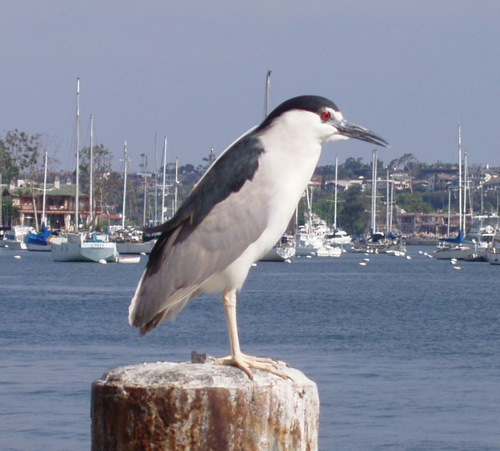
\includegraphics[width=.9\textwidth]{pavilion_bird_Black_Crowned_Night_Heron_01s.jpg}
\end{frame}

\begin{frame}
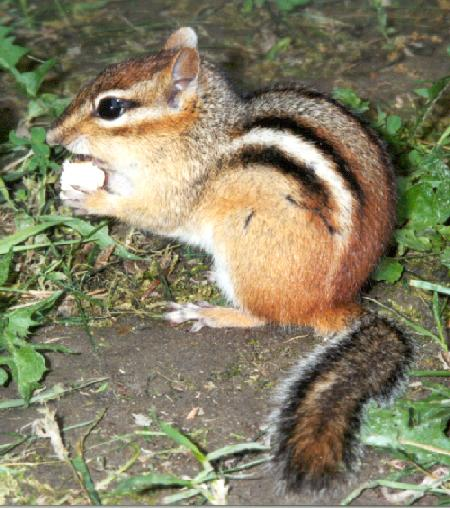
\includegraphics[width=.9\textwidth]{chipmunk1.jpg}
\end{frame}

\begin{frame}
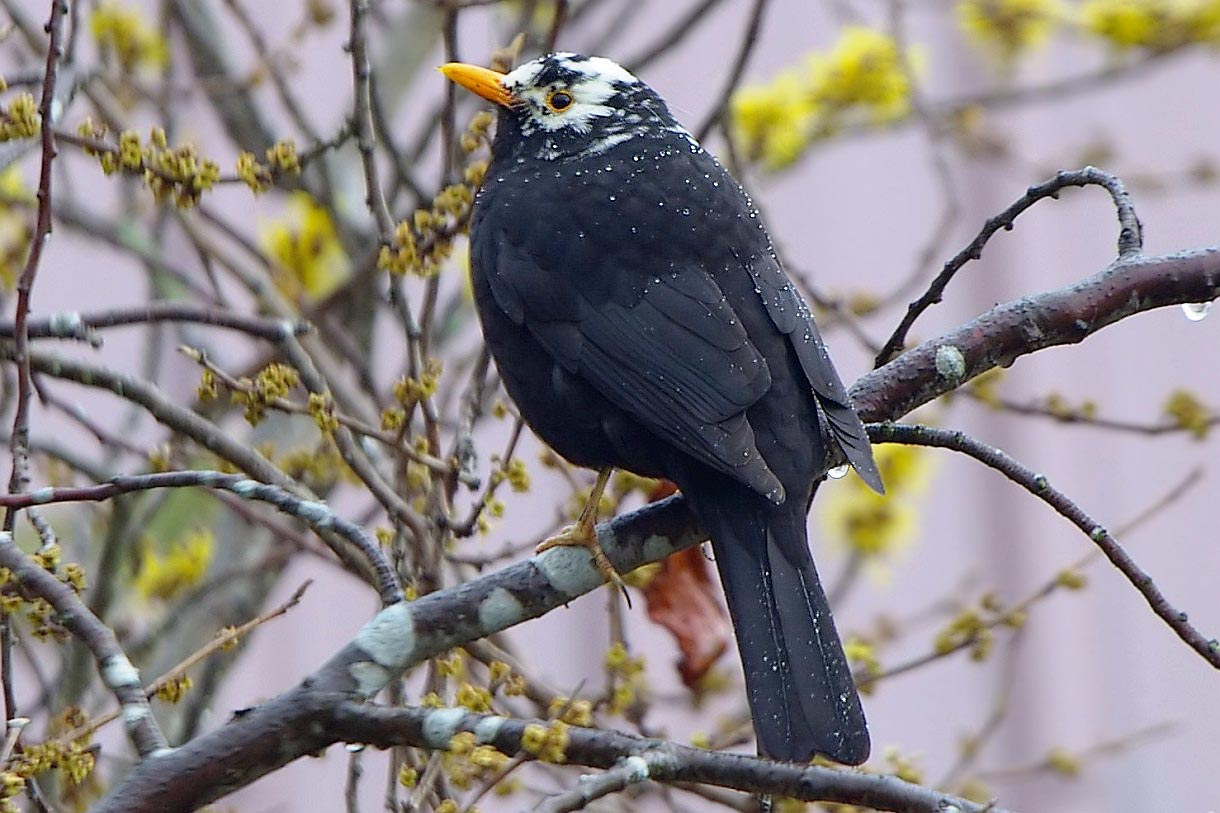
\includegraphics[width=.9\textwidth]{White-headed-Black-Bird.jpg}
\end{frame}

\begin{frame}
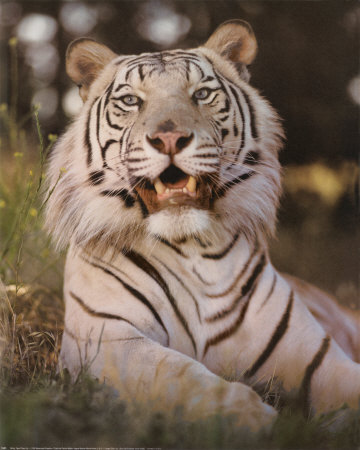
\includegraphics[width=.9\textwidth]{White-Tiger-Growling-Print-C10001340.jpg}
\end{frame}

\begin{frame}
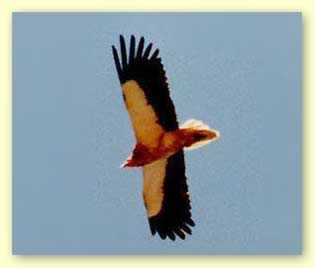
\includegraphics[width=.9\textwidth]{bird2.jpg}
\end{frame}

\begin{frame}
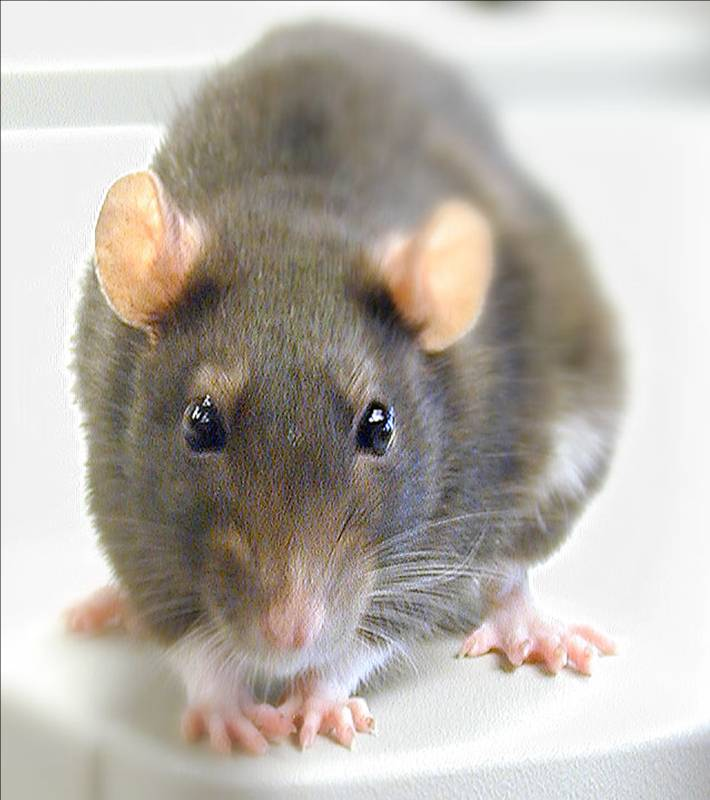
\includegraphics[width=.9\textwidth]{rat2.jpg}
\end{frame}

\begin{frame}
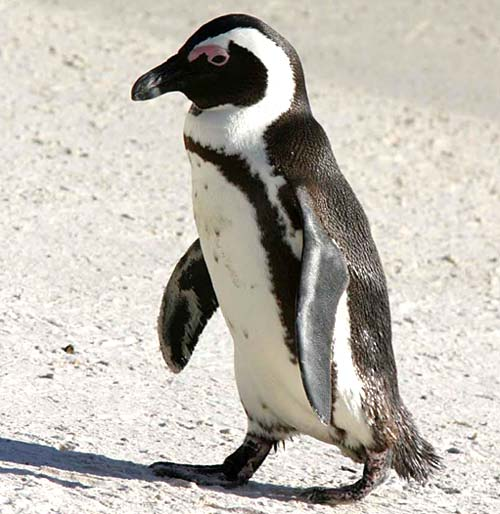
\includegraphics[width=.9\textwidth]{PenguinJck-Jul05CT-vertwl-w.jpg}
\end{frame}

\begin{frame}
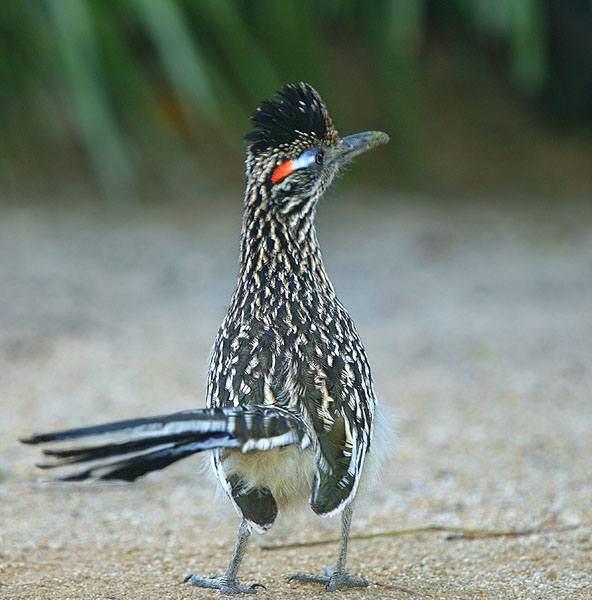
\includegraphics[width=.9\textwidth]{road-runner.jpg}
\end{frame}

\begin{frame}
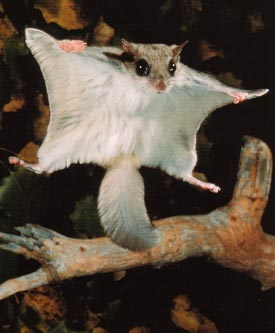
\includegraphics[width=.6\textwidth]{FlyingSquirrel.jpg}~~~~~~~~~~~~~~~~~~~~~~~~~~~~~~~~~~~~~~~~{\tiny ETEETETTEEE}
\end{frame}

\begin{frame}
\frametitle{What if I told you\dots}

\begin{tabular}{cc|cc|cc}
B & 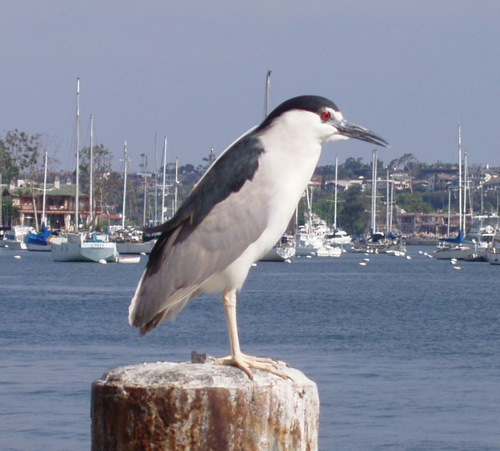
\includegraphics[width=.22\textwidth]{pavilion_bird_Black_Crowned_Night_Heron_01s.jpg}&
B & 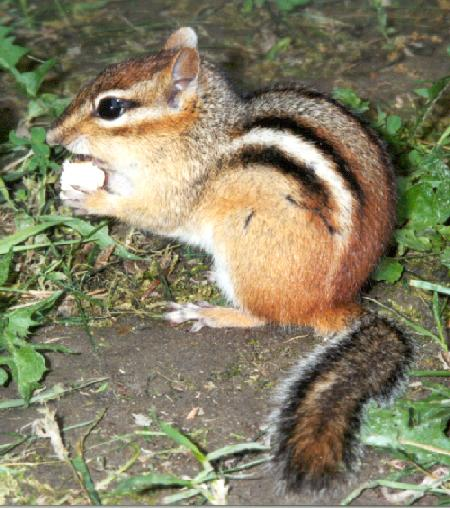
\includegraphics[width=.18\textwidth]{chipmunk1.jpg}&
A & 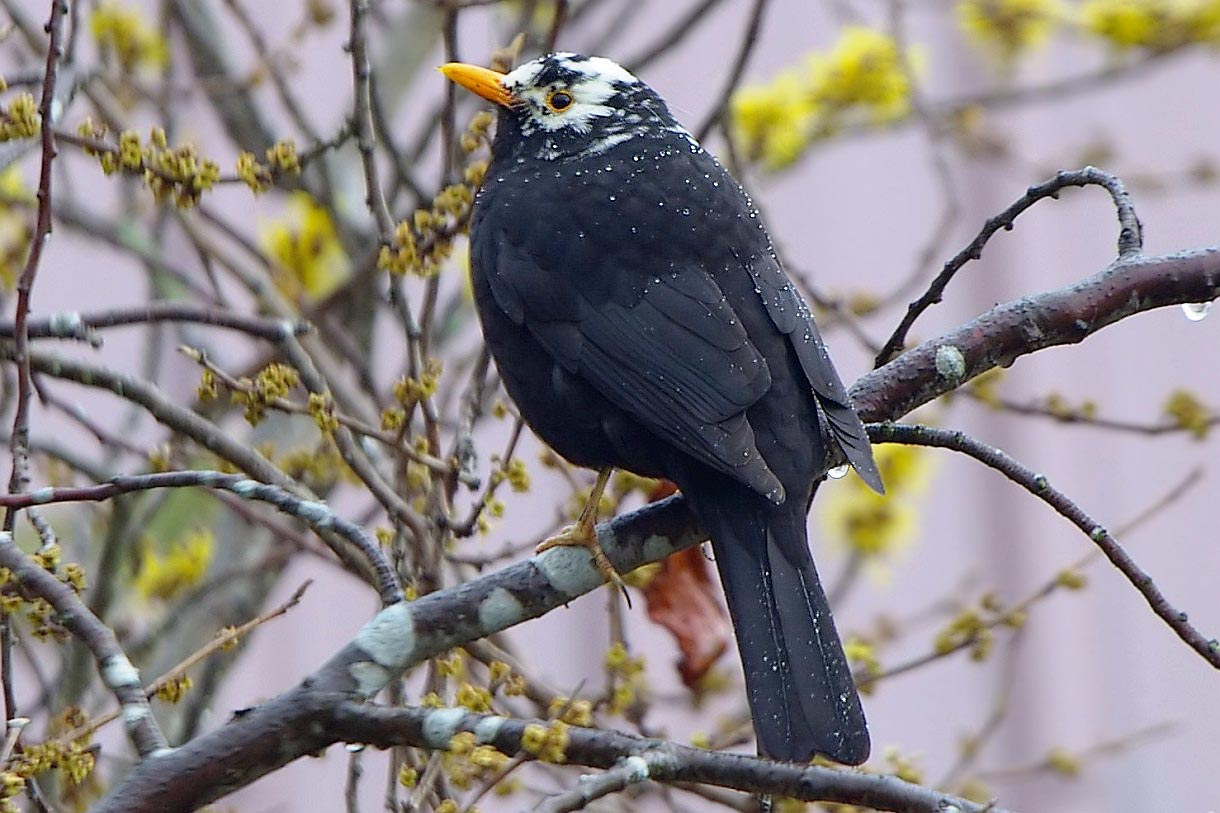
\includegraphics[width=.25\textwidth]{White-headed-Black-Bird.jpg}\\
\hline
B & 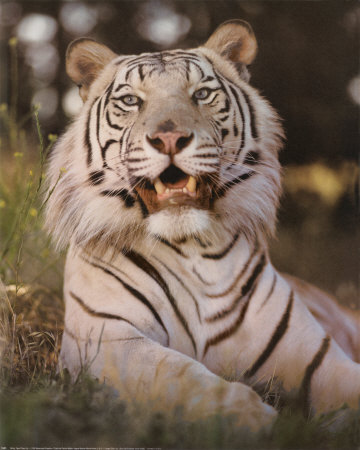
\includegraphics[width=.16\textwidth]{White-Tiger-Growling-Print-C10001340.jpg}&
A & 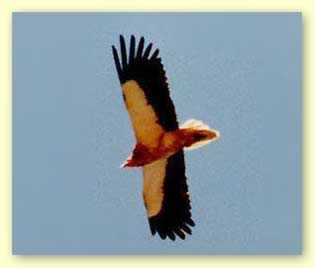
\includegraphics[width=.22\textwidth]{bird2.jpg}&
B & 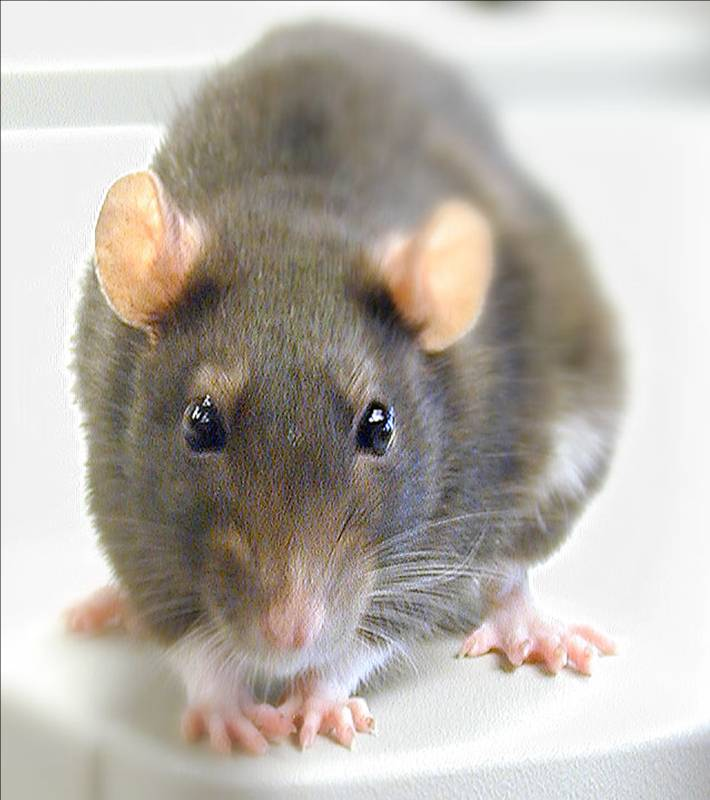
\includegraphics[width=.18\textwidth]{rat2.jpg}\\
\hline
B & 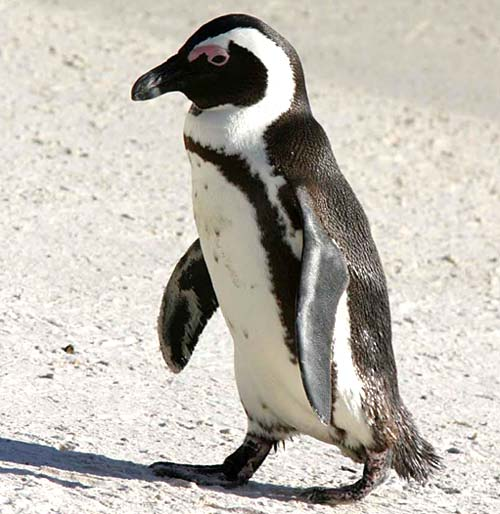
\includegraphics[width=.22\textwidth]{PenguinJck-Jul05CT-vertwl-w.jpg}&
A & 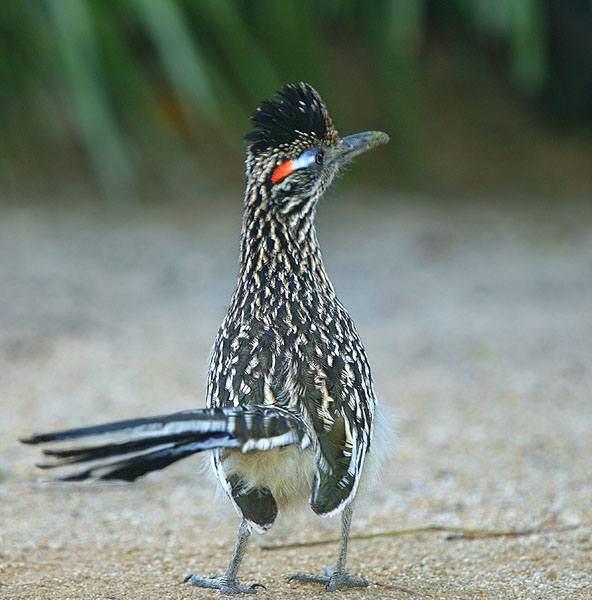
\includegraphics[width=.22\textwidth]{road-runner.jpg}&
A & 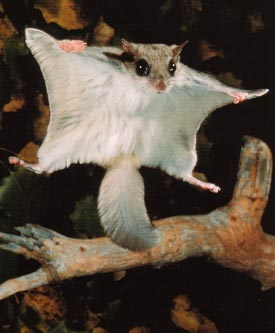
\includegraphics[width=.18\textwidth]{FlyingSquirrel.jpg}\\
\end{tabular}

\end{frame}


\end{document}
